\documentclass[12pt,a4paper]{article}

% if you need to pass options to natbib, use, e.g.:
%     \PassOptionsToPackage{numbers, compress}{natbib}
% before loading neurips_2022


% ready for submission
%\usepackage{ofu_xai_2022}

% SOURCE: https://github.com/goodfeli/dlbook_notation/blob/master/math_commands.tex
% Quote from github "We make them freely available for anyone to use."

\usepackage{amsmath,amsfonts,bm}


%%%%% NEW MATH DEFINITIONS %%%%%

% Mark sections of captions for referring to divisions of figures
\newcommand{\figleft}{{\em (Left)}}
\newcommand{\figcenter}{{\em (Center)}}
\newcommand{\figright}{{\em (Right)}}
\newcommand{\figtop}{{\em (Top)}}
\newcommand{\figbottom}{{\em (Bottom)}}
\newcommand{\captiona}{{\em (a)}}
\newcommand{\captionb}{{\em (b)}}
\newcommand{\captionc}{{\em (c)}}
\newcommand{\captiond}{{\em (d)}}

% Highlight a newly defined term
\newcommand{\newterm}[1]{{\bf #1}}


% Figure reference, lower-case.
\def\figref#1{figure~\ref{#1}}
% Figure reference, capital. For start of sentence
\def\Figref#1{Figure~\ref{#1}}
\def\twofigref#1#2{figures \ref{#1} and \ref{#2}}
\def\quadfigref#1#2#3#4{figures \ref{#1}, \ref{#2}, \ref{#3} and \ref{#4}}
% Section reference, lower-case.
\def\secref#1{section~\ref{#1}}
% Section reference, capital.
\def\Secref#1{Section~\ref{#1}}
% Reference to two sections.
\def\twosecrefs#1#2{sections \ref{#1} and \ref{#2}}
% Reference to three sections.
\def\secrefs#1#2#3{sections \ref{#1}, \ref{#2} and \ref{#3}}
% Reference to an equation, lower-case.
\def\eqref#1{equation~\ref{#1}}
% Reference to an equation, upper case
\def\Eqref#1{Equation~\ref{#1}}
% A raw reference to an equation---avoid using if possible
\def\plaineqref#1{\ref{#1}}
% Reference to a chapter, lower-case.
\def\chapref#1{chapter~\ref{#1}}
% Reference to an equation, upper case.
\def\Chapref#1{Chapter~\ref{#1}}
% Reference to a range of chapters
\def\rangechapref#1#2{chapters\ref{#1}--\ref{#2}}
% Reference to an algorithm, lower-case.
\def\algref#1{algorithm~\ref{#1}}
% Reference to an algorithm, upper case.
\def\Algref#1{Algorithm~\ref{#1}}
\def\twoalgref#1#2{algorithms \ref{#1} and \ref{#2}}
\def\Twoalgref#1#2{Algorithms \ref{#1} and \ref{#2}}
% Reference to a part, lower case
\def\partref#1{part~\ref{#1}}
% Reference to a part, upper case
\def\Partref#1{Part~\ref{#1}}
\def\twopartref#1#2{parts \ref{#1} and \ref{#2}}

\def\ceil#1{\lceil #1 \rceil}
\def\floor#1{\lfloor #1 \rfloor}
\def\1{\bm{1}}
\newcommand{\train}{\mathcal{D}}
\newcommand{\valid}{\mathcal{D_{\mathrm{valid}}}}
\newcommand{\test}{\mathcal{D_{\mathrm{test}}}}

\def\eps{{\epsilon}}


% Random variables
\def\reta{{\textnormal{$\eta$}}}
\def\ra{{\textnormal{a}}}
\def\rb{{\textnormal{b}}}
\def\rc{{\textnormal{c}}}
\def\rd{{\textnormal{d}}}
\def\re{{\textnormal{e}}}
\def\rf{{\textnormal{f}}}
\def\rg{{\textnormal{g}}}
\def\rh{{\textnormal{h}}}
\def\ri{{\textnormal{i}}}
\def\rj{{\textnormal{j}}}
\def\rk{{\textnormal{k}}}
\def\rl{{\textnormal{l}}}
% rm is already a command, just don't name any random variables m
\def\rn{{\textnormal{n}}}
\def\ro{{\textnormal{o}}}
\def\rp{{\textnormal{p}}}
\def\rq{{\textnormal{q}}}
\def\rr{{\textnormal{r}}}
\def\rs{{\textnormal{s}}}
\def\rt{{\textnormal{t}}}
\def\ru{{\textnormal{u}}}
\def\rv{{\textnormal{v}}}
\def\rw{{\textnormal{w}}}
\def\rx{{\textnormal{x}}}
\def\ry{{\textnormal{y}}}
\def\rz{{\textnormal{z}}}

% Random vectors
\def\rvepsilon{{\mathbf{\epsilon}}}
\def\rvtheta{{\mathbf{\theta}}}
\def\rva{{\mathbf{a}}}
\def\rvb{{\mathbf{b}}}
\def\rvc{{\mathbf{c}}}
\def\rvd{{\mathbf{d}}}
\def\rve{{\mathbf{e}}}
\def\rvf{{\mathbf{f}}}
\def\rvg{{\mathbf{g}}}
\def\rvh{{\mathbf{h}}}
\def\rvu{{\mathbf{i}}}
\def\rvj{{\mathbf{j}}}
\def\rvk{{\mathbf{k}}}
\def\rvl{{\mathbf{l}}}
\def\rvm{{\mathbf{m}}}
\def\rvn{{\mathbf{n}}}
\def\rvo{{\mathbf{o}}}
\def\rvp{{\mathbf{p}}}
\def\rvq{{\mathbf{q}}}
\def\rvr{{\mathbf{r}}}
\def\rvs{{\mathbf{s}}}
\def\rvt{{\mathbf{t}}}
\def\rvu{{\mathbf{u}}}
\def\rvv{{\mathbf{v}}}
\def\rvw{{\mathbf{w}}}
\def\rvx{{\mathbf{x}}}
\def\rvy{{\mathbf{y}}}
\def\rvz{{\mathbf{z}}}

% Elements of random vectors
\def\erva{{\textnormal{a}}}
\def\ervb{{\textnormal{b}}}
\def\ervc{{\textnormal{c}}}
\def\ervd{{\textnormal{d}}}
\def\erve{{\textnormal{e}}}
\def\ervf{{\textnormal{f}}}
\def\ervg{{\textnormal{g}}}
\def\ervh{{\textnormal{h}}}
\def\ervi{{\textnormal{i}}}
\def\ervj{{\textnormal{j}}}
\def\ervk{{\textnormal{k}}}
\def\ervl{{\textnormal{l}}}
\def\ervm{{\textnormal{m}}}
\def\ervn{{\textnormal{n}}}
\def\ervo{{\textnormal{o}}}
\def\ervp{{\textnormal{p}}}
\def\ervq{{\textnormal{q}}}
\def\ervr{{\textnormal{r}}}
\def\ervs{{\textnormal{s}}}
\def\ervt{{\textnormal{t}}}
\def\ervu{{\textnormal{u}}}
\def\ervv{{\textnormal{v}}}
\def\ervw{{\textnormal{w}}}
\def\ervx{{\textnormal{x}}}
\def\ervy{{\textnormal{y}}}
\def\ervz{{\textnormal{z}}}

% Random matrices
\def\rmA{{\mathbf{A}}}
\def\rmB{{\mathbf{B}}}
\def\rmC{{\mathbf{C}}}
\def\rmD{{\mathbf{D}}}
\def\rmE{{\mathbf{E}}}
\def\rmF{{\mathbf{F}}}
\def\rmG{{\mathbf{G}}}
\def\rmH{{\mathbf{H}}}
\def\rmI{{\mathbf{I}}}
\def\rmJ{{\mathbf{J}}}
\def\rmK{{\mathbf{K}}}
\def\rmL{{\mathbf{L}}}
\def\rmM{{\mathbf{M}}}
\def\rmN{{\mathbf{N}}}
\def\rmO{{\mathbf{O}}}
\def\rmP{{\mathbf{P}}}
\def\rmQ{{\mathbf{Q}}}
\def\rmR{{\mathbf{R}}}
\def\rmS{{\mathbf{S}}}
\def\rmT{{\mathbf{T}}}
\def\rmU{{\mathbf{U}}}
\def\rmV{{\mathbf{V}}}
\def\rmW{{\mathbf{W}}}
\def\rmX{{\mathbf{X}}}
\def\rmY{{\mathbf{Y}}}
\def\rmZ{{\mathbf{Z}}}

% Elements of random matrices
\def\ermA{{\textnormal{A}}}
\def\ermB{{\textnormal{B}}}
\def\ermC{{\textnormal{C}}}
\def\ermD{{\textnormal{D}}}
\def\ermE{{\textnormal{E}}}
\def\ermF{{\textnormal{F}}}
\def\ermG{{\textnormal{G}}}
\def\ermH{{\textnormal{H}}}
\def\ermI{{\textnormal{I}}}
\def\ermJ{{\textnormal{J}}}
\def\ermK{{\textnormal{K}}}
\def\ermL{{\textnormal{L}}}
\def\ermM{{\textnormal{M}}}
\def\ermN{{\textnormal{N}}}
\def\ermO{{\textnormal{O}}}
\def\ermP{{\textnormal{P}}}
\def\ermQ{{\textnormal{Q}}}
\def\ermR{{\textnormal{R}}}
\def\ermS{{\textnormal{S}}}
\def\ermT{{\textnormal{T}}}
\def\ermU{{\textnormal{U}}}
\def\ermV{{\textnormal{V}}}
\def\ermW{{\textnormal{W}}}
\def\ermX{{\textnormal{X}}}
\def\ermY{{\textnormal{Y}}}
\def\ermZ{{\textnormal{Z}}}

% Vectors
\def\vzero{{\bm{0}}}
\def\vone{{\bm{1}}}
\def\vmu{{\bm{\mu}}}
\def\vtheta{{\bm{\theta}}}
\def\va{{\bm{a}}}
\def\vb{{\bm{b}}}
\def\vc{{\bm{c}}}
\def\vd{{\bm{d}}}
\def\ve{{\bm{e}}}
\def\vf{{\bm{f}}}
\def\vg{{\bm{g}}}
\def\vh{{\bm{h}}}
\def\vi{{\bm{i}}}
\def\vj{{\bm{j}}}
\def\vk{{\bm{k}}}
\def\vl{{\bm{l}}}
\def\vm{{\bm{m}}}
\def\vn{{\bm{n}}}
\def\vo{{\bm{o}}}
\def\vp{{\bm{p}}}
\def\vq{{\bm{q}}}
\def\vr{{\bm{r}}}
\def\vs{{\bm{s}}}
\def\vt{{\bm{t}}}
\def\vu{{\bm{u}}}
\def\vv{{\bm{v}}}
\def\vw{{\bm{w}}}
\def\vx{{\bm{x}}}
\def\vy{{\bm{y}}}
\def\vz{{\bm{z}}}

% Elements of vectors
\def\evalpha{{\alpha}}
\def\evbeta{{\beta}}
\def\evepsilon{{\epsilon}}
\def\evlambda{{\lambda}}
\def\evomega{{\omega}}
\def\evmu{{\mu}}
\def\evpsi{{\psi}}
\def\evsigma{{\sigma}}
\def\evtheta{{\theta}}
\def\eva{{a}}
\def\evb{{b}}
\def\evc{{c}}
\def\evd{{d}}
\def\eve{{e}}
\def\evf{{f}}
\def\evg{{g}}
\def\evh{{h}}
\def\evi{{i}}
\def\evj{{j}}
\def\evk{{k}}
\def\evl{{l}}
\def\evm{{m}}
\def\evn{{n}}
\def\evo{{o}}
\def\evp{{p}}
\def\evq{{q}}
\def\evr{{r}}
\def\evs{{s}}
\def\evt{{t}}
\def\evu{{u}}
\def\evv{{v}}
\def\evw{{w}}
\def\evx{{x}}
\def\evy{{y}}
\def\evz{{z}}

% Matrix
\def\mA{{\bm{A}}}
\def\mB{{\bm{B}}}
\def\mC{{\bm{C}}}
\def\mD{{\bm{D}}}
\def\mE{{\bm{E}}}
\def\mF{{\bm{F}}}
\def\mG{{\bm{G}}}
\def\mH{{\bm{H}}}
\def\mI{{\bm{I}}}
\def\mJ{{\bm{J}}}
\def\mK{{\bm{K}}}
\def\mL{{\bm{L}}}
\def\mM{{\bm{M}}}
\def\mN{{\bm{N}}}
\def\mO{{\bm{O}}}
\def\mP{{\bm{P}}}
\def\mQ{{\bm{Q}}}
\def\mR{{\bm{R}}}
\def\mS{{\bm{S}}}
\def\mT{{\bm{T}}}
\def\mU{{\bm{U}}}
\def\mV{{\bm{V}}}
\def\mW{{\bm{W}}}
\def\mX{{\bm{X}}}
\def\mY{{\bm{Y}}}
\def\mZ{{\bm{Z}}}
\def\mBeta{{\bm{\beta}}}
\def\mPhi{{\bm{\Phi}}}
\def\mLambda{{\bm{\Lambda}}}
\def\mSigma{{\bm{\Sigma}}}

% Tensor
\DeclareMathAlphabet{\mathsfit}{\encodingdefault}{\sfdefault}{m}{sl}
\SetMathAlphabet{\mathsfit}{bold}{\encodingdefault}{\sfdefault}{bx}{n}
\newcommand{\tens}[1]{\bm{\mathsfit{#1}}}
\def\tA{{\tens{A}}}
\def\tB{{\tens{B}}}
\def\tC{{\tens{C}}}
\def\tD{{\tens{D}}}
\def\tE{{\tens{E}}}
\def\tF{{\tens{F}}}
\def\tG{{\tens{G}}}
\def\tH{{\tens{H}}}
\def\tI{{\tens{I}}}
\def\tJ{{\tens{J}}}
\def\tK{{\tens{K}}}
\def\tL{{\tens{L}}}
\def\tM{{\tens{M}}}
\def\tN{{\tens{N}}}
\def\tO{{\tens{O}}}
\def\tP{{\tens{P}}}
\def\tQ{{\tens{Q}}}
\def\tR{{\tens{R}}}
\def\tS{{\tens{S}}}
\def\tT{{\tens{T}}}
\def\tU{{\tens{U}}}
\def\tV{{\tens{V}}}
\def\tW{{\tens{W}}}
\def\tX{{\tens{X}}}
\def\tY{{\tens{Y}}}
\def\tZ{{\tens{Z}}}


% Graph
\def\gA{{\mathcal{A}}}
\def\gB{{\mathcal{B}}}
\def\gC{{\mathcal{C}}}
\def\gD{{\mathcal{D}}}
\def\gE{{\mathcal{E}}}
\def\gF{{\mathcal{F}}}
\def\gG{{\mathcal{G}}}
\def\gH{{\mathcal{H}}}
\def\gI{{\mathcal{I}}}
\def\gJ{{\mathcal{J}}}
\def\gK{{\mathcal{K}}}
\def\gL{{\mathcal{L}}}
\def\gM{{\mathcal{M}}}
\def\gN{{\mathcal{N}}}
\def\gO{{\mathcal{O}}}
\def\gP{{\mathcal{P}}}
\def\gQ{{\mathcal{Q}}}
\def\gR{{\mathcal{R}}}
\def\gS{{\mathcal{S}}}
\def\gT{{\mathcal{T}}}
\def\gU{{\mathcal{U}}}
\def\gV{{\mathcal{V}}}
\def\gW{{\mathcal{W}}}
\def\gX{{\mathcal{X}}}
\def\gY{{\mathcal{Y}}}
\def\gZ{{\mathcal{Z}}}

% Sets
\def\sA{{\mathbb{A}}}
\def\sB{{\mathbb{B}}}
\def\sC{{\mathbb{C}}}
\def\sD{{\mathbb{D}}}
% Don't use a set called E, because this would be the same as our symbol
% for expectation.
\def\sF{{\mathbb{F}}}
\def\sG{{\mathbb{G}}}
\def\sH{{\mathbb{H}}}
\def\sI{{\mathbb{I}}}
\def\sJ{{\mathbb{J}}}
\def\sK{{\mathbb{K}}}
\def\sL{{\mathbb{L}}}
\def\sM{{\mathbb{M}}}
\def\sN{{\mathbb{N}}}
\def\sO{{\mathbb{O}}}
\def\sP{{\mathbb{P}}}
\def\sQ{{\mathbb{Q}}}
\def\sR{{\mathbb{R}}}
\def\sS{{\mathbb{S}}}
\def\sT{{\mathbb{T}}}
\def\sU{{\mathbb{U}}}
\def\sV{{\mathbb{V}}}
\def\sW{{\mathbb{W}}}
\def\sX{{\mathbb{X}}}
\def\sY{{\mathbb{Y}}}
\def\sZ{{\mathbb{Z}}}

% Entries of a matrix
\def\emLambda{{\Lambda}}
\def\emA{{A}}
\def\emB{{B}}
\def\emC{{C}}
\def\emD{{D}}
\def\emE{{E}}
\def\emF{{F}}
\def\emG{{G}}
\def\emH{{H}}
\def\emI{{I}}
\def\emJ{{J}}
\def\emK{{K}}
\def\emL{{L}}
\def\emM{{M}}
\def\emN{{N}}
\def\emO{{O}}
\def\emP{{P}}
\def\emQ{{Q}}
\def\emR{{R}}
\def\emS{{S}}
\def\emT{{T}}
\def\emU{{U}}
\def\emV{{V}}
\def\emW{{W}}
\def\emX{{X}}
\def\emY{{Y}}
\def\emZ{{Z}}
\def\emSigma{{\Sigma}}

% entries of a tensor
% Same font as tensor, without \bm wrapper
\newcommand{\etens}[1]{\mathsfit{#1}}
\def\etLambda{{\etens{\Lambda}}}
\def\etA{{\etens{A}}}
\def\etB{{\etens{B}}}
\def\etC{{\etens{C}}}
\def\etD{{\etens{D}}}
\def\etE{{\etens{E}}}
\def\etF{{\etens{F}}}
\def\etG{{\etens{G}}}
\def\etH{{\etens{H}}}
\def\etI{{\etens{I}}}
\def\etJ{{\etens{J}}}
\def\etK{{\etens{K}}}
\def\etL{{\etens{L}}}
\def\etM{{\etens{M}}}
\def\etN{{\etens{N}}}
\def\etO{{\etens{O}}}
\def\etP{{\etens{P}}}
\def\etQ{{\etens{Q}}}
\def\etR{{\etens{R}}}
\def\etS{{\etens{S}}}
\def\etT{{\etens{T}}}
\def\etU{{\etens{U}}}
\def\etV{{\etens{V}}}
\def\etW{{\etens{W}}}
\def\etX{{\etens{X}}}
\def\etY{{\etens{Y}}}
\def\etZ{{\etens{Z}}}

% The true underlying data generating distribution
\newcommand{\pdata}{p_{\rm{data}}}
% The empirical distribution defined by the training set
\newcommand{\ptrain}{\hat{p}_{\rm{data}}}
\newcommand{\Ptrain}{\hat{P}_{\rm{data}}}
% The model distribution
\newcommand{\pmodel}{p_{\rm{model}}}
\newcommand{\Pmodel}{P_{\rm{model}}}
\newcommand{\ptildemodel}{\tilde{p}_{\rm{model}}}
% Stochastic autoencoder distributions
\newcommand{\pencode}{p_{\rm{encoder}}}
\newcommand{\pdecode}{p_{\rm{decoder}}}
\newcommand{\precons}{p_{\rm{reconstruct}}}

\newcommand{\laplace}{\mathrm{Laplace}} % Laplace distribution

\newcommand{\E}{\mathbb{E}}
\newcommand{\Ls}{\mathcal{L}}
\newcommand{\R}{\mathbb{R}}
\newcommand{\emp}{\tilde{p}}
\newcommand{\lr}{\alpha}
\newcommand{\reg}{\lambda}
\newcommand{\rect}{\mathrm{rectifier}}
\newcommand{\softmax}{\mathrm{softmax}}
\newcommand{\sigmoid}{\sigma}
\newcommand{\softplus}{\zeta}
\newcommand{\KL}{D_{\mathrm{KL}}}
\newcommand{\Var}{\mathrm{Var}}
\newcommand{\standarderror}{\mathrm{SE}}
\newcommand{\Cov}{\mathrm{Cov}}
% Wolfram Mathworld says $L^2$ is for function spaces and $\ell^2$ is for vectors
% But then they seem to use $L^2$ for vectors throughout the site, and so does
% wikipedia.
\newcommand{\normlzero}{L^0}
\newcommand{\normlone}{L^1}
\newcommand{\normltwo}{L^2}
\newcommand{\normlp}{L^p}
\newcommand{\normmax}{L^\infty}

\newcommand{\parents}{Pa} % See usage in notation.tex. Chosen to match Daphne's book.

%\DeclareMathOperator*{\argmax}{arg\,max}
%\DeclareMathOperator*{\argmin}{arg\,min}

%\DeclareMathOperator{\sign}{sign}
%\DeclareMathOperator{\Tr}{Tr}
\let\ab\allowbreak

% to compile a preprint version, e.g., for submission to arXiv, add add the
% [preprint] option:
%     \usepackage[preprint]{ofu_xai_2022}


% to compile a camera-ready version, add the [final] option, e.g.:
\usepackage[final, nonatbib]{ofu_xai_2022}

% to avoid loading the natbib package, add option nonatbib:
%    \usepackage[nonatbib]{ofu_xai_2022}


\usepackage[utf8]{inputenc} % allow utf-8 input
\usepackage[T1]{fontenc}    % use 8-bit T1 fonts
\usepackage{hyperref}       % hyperlinks
\usepackage{url}            % simple URL typesetting
\usepackage{booktabs}       % professional-quality tables
\usepackage{amsfonts}       % blackboard math symbols
\usepackage{nicefrac}       % compact symbols for 1/2, etc.
\usepackage{microtype}      % microtypography
\usepackage{xcolor}         % colors
\usepackage{setspace}
\usepackage{titlesec}
\usepackage[utf8]{inputenc}
%\usepackage{biblatex}
\usepackage{wrapfig}
\usepackage{hyperref}
\usepackage{ragged2e}
\usepackage{multicol}
\usepackage{graphicx}
\titlespacing{\title}{0pt}{\parskip}{-\parskip}
\titlespacing{\section}{0.5pt}{\parskip}{-\parskip}
\linespread{1.5}

\usepackage[round]{natbib}
%%%%

\title{ KuchBhiRakhDo \\ {\large xAI-Proj-B: Bachelor Project Explainable Machine Learning } \\ {\large A Semester in the Life of a Deep Learning Engineer}}


% The \author macro works with any number of authors. There are two commands
% used to separate the names and addresses of multiple authors: \And and \AND.
%
% Using \And between authors leaves it to LaTeX to determine where to break the
% lines. Using \AND forces a line break at that point. So, if LaTeX puts 3 of 4
% authors names on the first line, and the last on the second line, try using
% \AND instead of \And before the third author name.


\author{%
  Shehroz Shafiq Khan\thanks{Degree: M.Sc. International Software System Science, matriculation \#: 2093254} \\
  Otto-Friedrich University of Bamberg\\
  96049 Bamberg, Germany\\
  \texttt{shehroz.shafiq-khan@stud.uni-bamberg.de}\\
  % examples of more authors
   \And
   Hafiz Ahmer Saeed Khan\thanks{Degree: M.Sc. International Software System Science, matriculation \#: 2092973}\\
   Otto-Friedrich University of Bamberg\\
   96049 Bamberg, Germany\\
   \texttt{hafiz.ahmer.saeed-khan@stud.uni-bamberg.de} \\
   \And
   Muhammad Junaid\thanks{Degree: M.Sc. International Software System Science, matriculation \#: 2097636}\\
   Otto-Friedrich University of Bamberg\\
   96049 Bamberg, Germany\\
   \texttt{muhammad.junaid@stud.uni-bamberg.de} \\
  % \And
  % Coauthor \\
  % Affiliation \\
  % Address \\
  % \texttt{email} \\
  % \And
  % Coauthor \\
  % Affiliation \\
  % Address \\
  % \texttt{email} \\
}


\begin{document}


\maketitle
\def\va{{\bm{a}}}
\pagebreak
\begin{abstract}
In this project, we combined the power of deep learning techniques to excel in recognizing single-digit numbers. Our project consists of two main parts, each focusing on different datasets and architectures. In the first part, we explored the MNIST dataset, which contains a large collection of handwritten digits. We trained a customized Convolutional Neural Network (CNN) to accurately understand the intricacies of these handwritten digits. In the second part, we explored street house numbers captured in real-world images. We used the VGG-16 architecture and around 700 images to successfully recognize these street digits with high accuracy. This shows that our techniques work well in different areas. Our work combines technology and perception to achieve successful recognition of single-digit numbers. We've put all our work in our Git repository so others can see and learn from it: \url{https://github.com/shehrozshafiqkh/xAI-deep-learning}
\end{abstract}


\section{Introduction}

\textbf{"A semester in life of a Deep learning Engineer".}

We're showing a cool mix of machine learning and computer vision. Our aim is to figure out the secret of spotting single numbers using deep learning techniques.

We started with a well-known dataset of handwritten numbers called MNIST. People who like computers and pictures have loved this for a long time. We've used deep learning techniques that use Convolutional Neural Networks (CNN) to get the numbers right and also to understand why they look the way they do.

But we did not just stick to computers but also went to real street house numbers where there are single numbers on signs. We got ideas from colorful pictures and used a popular CNN architecture called VGG-16 to predict these street numbers.

%\pagebreak

\subsection{Background}
In this project, we tackled 2 problems regarding single-digit recognition using MNIST and Street Numbers datasets.

\subsubsection{MNIST}
The MNIST dataset is a widely used collection of handwritten digit images commonly employed for machine learning and computer vision tasks. It contains a set of 28x28 grayscale images, each depicting a single digit from 0 to 9. The dataset is divided into two main parts: a training set and a test set. 

The training set consists of thousands of images, where each image is labeled with its corresponding digit (0 to 9). Machine learning models can use this labeled data to learn the patterns and characteristics of each digit. The model can then use this learned knowledge to predict the digit in new, unseen images. 

The test set serves as a benchmark to evaluate the model's performance. It contains images that the model has never encountered during training. The model's predictions are compared to the actual labels of the test images to measure its accuracy. 

The MNIST dataset is commonly used to develop and test various machine learning algorithms, especially for image classification tasks. It's a fundamental resource for researchers and practitioners to assess the effectiveness of different techniques in the realm of digit recognition and image analysis.

\subsubsection{Street Numbers}
We gathered the StreetNumbers dataset firsthand by venturing into various neighborhoods across Bamberg. Our group with other teams captured a collection of over 700 high-resolution images. These images were initially in high resolution and were subsequently resized to dimensions of 256 by 256 pixels. All pictures were in RGB format. These images represent real-world scenarios and feature numbers displayed on signs and buildings. The primary objective of utilizing this dataset was to evaluate the performance of our pre-existing model on authentic, real-world data. 

Utilizing cutting-edge neural networks, we embarked on the mission of training our system to visually comprehend and identify street house numbers.

\subsection{Related Work}
We have extensively reviewed and analyzed two prominent research papers. These comprehensive studies have significantly contributed to our understanding of the domain of deep learning and provided valuable insights into the topic.

\begin{itemize}
    \item Very Deep Convolutional Networks for Large-Scale Image Recognition
    \newline \url{https://arxiv.org/abs/1409.1556}
    \newline Karen Simonyan, Andrew Zisserman

    \item Deep Residual Learning for Image Recognition
    \newline \url{https://arxiv.org/abs/1512.03385}
    \newline Kaiming He, Xiangyu Zhang, Shaoqing Ren, Jian Sun
\end{itemize}

\subsection{Contribution}
Throughout this project, our main objective was to develop a robust solution for accurately recognizing single-digit numbers using deep learning techniques. We have made significant contributions in terms of innovative methodologies and practical implementations that push the boundaries of the current state of the art in this field.
\linebreak
\linebreak

Here is an overview of our achievements:

We extensively explored cloud-based training platforms, such as GCP and Google Colab, seamlessly integrating them into our model training process. This integration allowed us to efficiently utilize substantial computational resources for experimenting with intricate neural network architectures.

To counter overfitting challenges, we introduced inventive data augmentation techniques, including rotation, flipping, and cropping. By strategically enhancing our training dataset, we significantly improved our models' ability to generalize effectively across diverse real-world data.

By leveraging Keras's transfer learning capabilities, we seamlessly integrated pre-trained models like VGG-16 into our framework. This accelerated the training process and allowed us to transfer valuable features from extensive datasets to our specific problem domain.

We conducted exhaustive experiments to explore the robustness and reliability of our models. These experiments rigorously evaluated the models' ability to handle diverse inputs and ensured consistent performance under varying conditions, increasing the overall reliability and performance of our model.

\linebreak
%\pagebreak

\section{Methods}
\subsection{First Approach}
In our first approach, we constructed a Convolutional Neural Network (CNN) using Keras. The model begins with a convolutional layer involving 28 filters with a 3x3 kernel size, extracting features from input images. A subsequent max pooling layer reduces feature map dimensions, aiding computational efficiency. The flattened data is then processed by a dense layer with 128 neurons and ReLU activation. A dropout layer with a 20\% deactivation rate helps prevent overfitting. Finally, a 10-neuron output layer with softmax activation produces class probabilities for classification tasks. This design is commonly used for image analysis, effectively extracting features and making predictions based on them.

\begin{figure}[h]
    \centering
    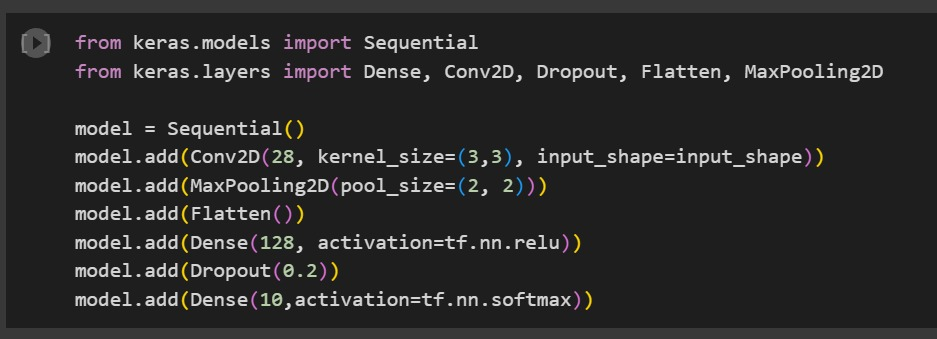
\includegraphics[width=\linewidth]{images/2.1 Testing.jpeg}
     
     
     \caption{}     \label{fig:my_label} 
    \end{figure}\\

\subsection{Second Approach}
In our second approach, the initial step involved loading the pre-trained VGG-16 model, excluding its top classification layers. This model, trained on the 'imagenet' dataset, is designed to extract intricate features from images. The input shape was defined as (256, 256, 3), indicating an image size of 256x256 pixels with 3 color channels (RGB).

We then froze the weights of the pre-trained layers to retain the previously learned features. A new sequential model was instantiated using Keras and the pre-trained VGG-16 layers were added to it. That formed the foundation for feature extraction from input images.

To adapt the VGG-16 layers for the specific classification task, extra layers were appended. First, a 'Flatten' layer reshaped the extracted features into a vector. Then, a dense layer with 256 neurons, employing the rectified linear unit (ReLU) activation function, contributed to feature transformation. Another dense layer with 10 neurons and softmax activation facilitated multi-class classification.

\begin{figure}[h]
    \centering
    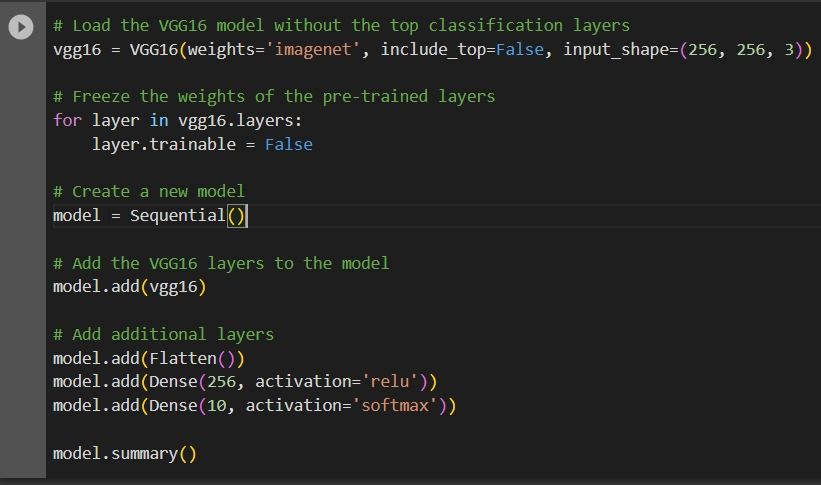
\includegraphics[width=\linewidth]{images/Summary.jpeg}
     
     
     \caption{}     \label{fig:my_label} 
    \end{figure}\\
%\pagebreak

\section{Experiments and Results}
\subsection{Used Dataset}
\begin{multicols}{2}
\textbf{→ MNIST dataset}
\begin{itemize}
    \item 70.000 images
    \item 28 X 28 Pixels
    \item Grayscale
\end{itemize}
\linebreak
\newline
\textbf{→ Streetnumber Dataset}
\begin{itemize}
    \item 714 images
    \item 256 X 256 Pixels
    \item RGB
\end{itemize}
\end{multicols}


\subsection{Experimental Setup}


\begin{itemize}
    \item Experimental setup Model from scratch → Switch to VGG-16
    \item Learning rate adjustments
    \item Hyperparameter optimization
\end{itemize} 

This experimental setup aims to enhance the performance of a machine-learning model for a specific task, such as image classification. The process is divided into two phases: creating a model from scratch and then switching to a pre-trained VGG-16 model, a commonly used deep neural network architecture. Initially, a custom model is built by designing layers like convolutional, pooling, and fully connected layers. After evaluating the scratch model's effectiveness, the experiment then shifts to utilizing the VGG-16 model, which has already been trained on a vast dataset for general image recognition tasks. This pre-trained model can potentially offer superior initial features and representations for the specific task. The learning rate is another factor adjusted to optimize the process. The learning rate identifies the step size taken in updating the model's parameters during training. By fine-tuning this hyperparameter, the goal is to strike the right balance between swift convergence and bypassing overshooting the optimal values. This iterative approach of transitioning from a custom model to a pre-trained one and tuning the learning rates represents a purposeful strategy to improve model performance, combining architectural know-how and hyperparameter refinement to achieve superior results.

%\pagebreak

\subsection{Hyperparameter Tuning Results}

Figure 3 illustrates the iterative process of training our model using 5 epochs and 8 batch sizes. Within each epoch, the model processes batches of 8 data points. It starts with a forward pass, making predictions based on input data. These predictions are compared to actual values to calculate a loss, representing performance. Backpropagation then adjusts model parameters to minimize the loss. This weight update refines predictions, iteratively improving the model's understanding through each batch. As epochs progress, the model's predictions converge towards accurate values, signifying enhanced performance.

\begin{figure}[h]
    \centering
    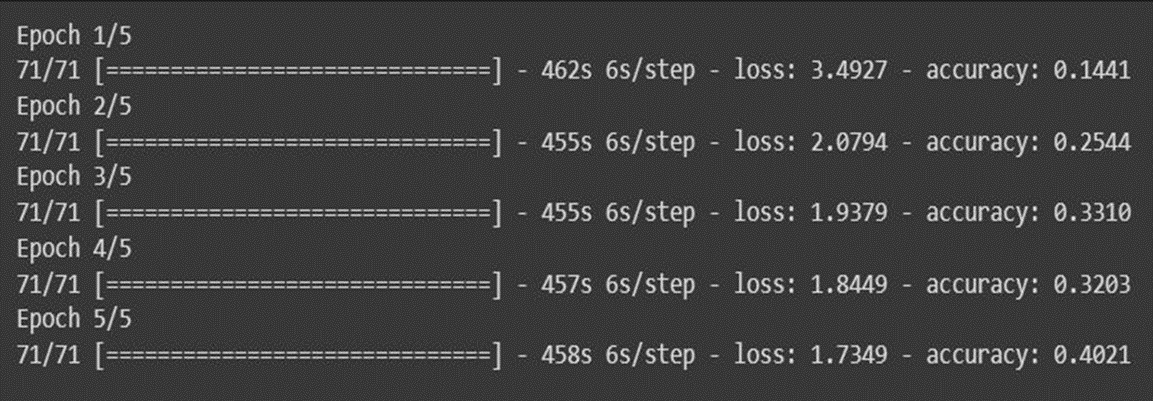
\includegraphics[width=\linewidth]{images/3.3.1.jpeg}
     
     
     \caption{}     \label{fig:my_label} 
    \end{figure}\\

In Figure 4 below, we maintained the 5 epochs from the prior training procedure, but this time, we scaled up the batch size from 8 to 16.
    
\begin{figure}[h]
    \centering
    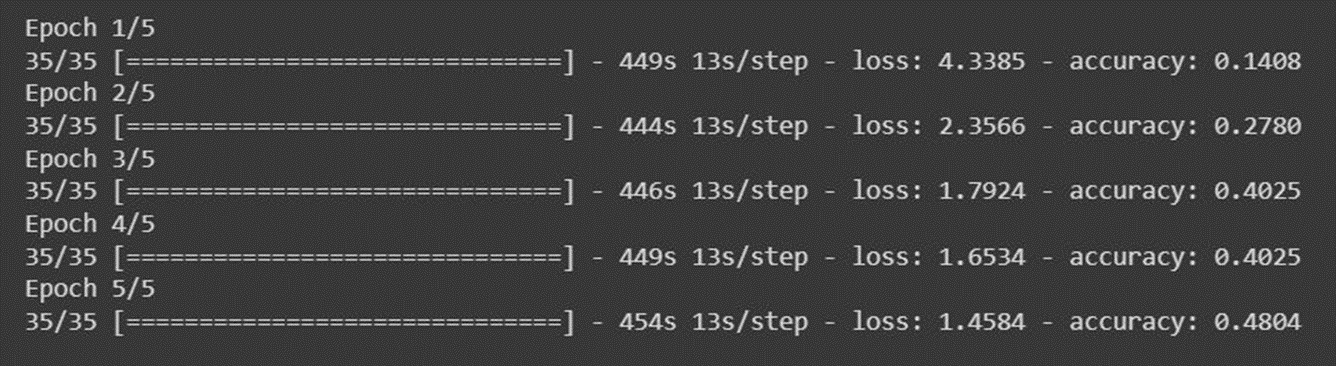
\includegraphics[width=\linewidth]{images/3.3.2.jpeg}
     
     
     \caption{}     \label{fig:my_label} 
    \end{figure}\\

%\pagebreak
Moving on to Figure 5, we extended our training epochs to 10 and adjusted the batch size to 16. This alteration aimed to gauge the convergence of our model. Our observations align with previous instances where modifying these values impacted the training outcome. Notably, the results confirmed this effect, as these parameter adjustments produced the highest accuracy among the preceding cases.

\begin{figure}[h]
    \centering
    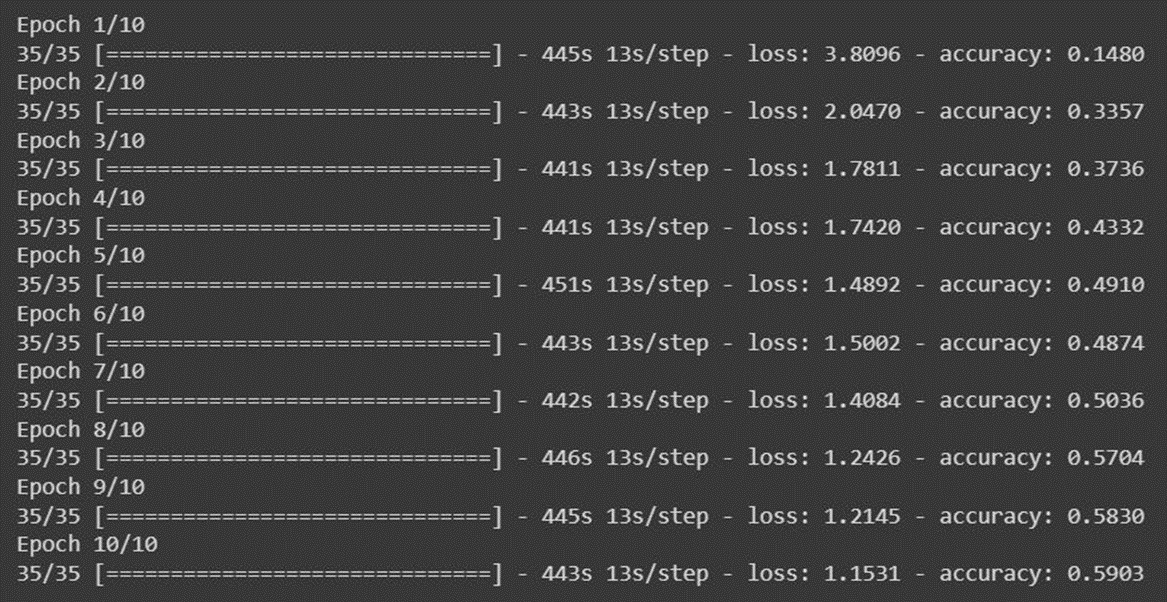
\includegraphics[width=\linewidth]{images/3.3.3.jpeg}
     
     
     \caption{}     \label{fig:my_label} 
    \end{figure}\\
\pagebreak
\subsection{Results}

Figure 6 depicts a consistent trend: the accuracy of our model rises with the increasing number of training epochs. This pattern suggests that our model is progressively improving its predictive performance as it undergoes more training iterations. The climbing accuracy signifies that our model is successfully learning and adapting to the dataset, becoming more skilled at making accurate predictions.

\begin{figure}[h]
    \centering
    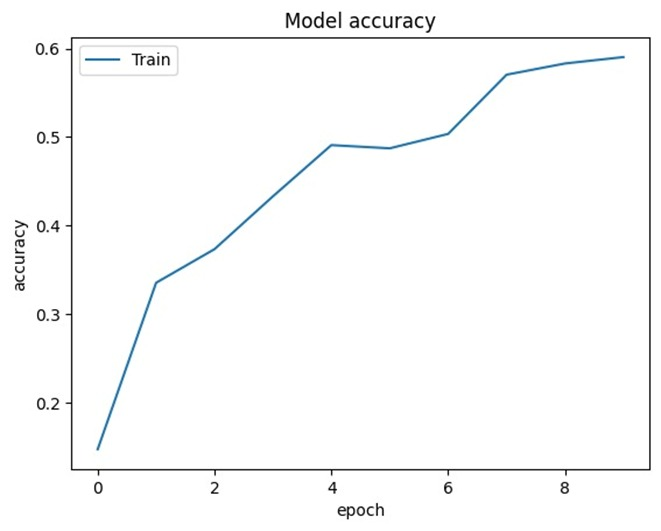
\includegraphics[width=\linewidth]{images/3.4.1.jpeg}
     
     
     \caption{}     \label{fig:my_label} 
    \end{figure}\\

\pagebreak 
In Figure 7 below, our model's loss decreases with each epoch, which signifies that the model's predictions are becoming progressively more accurate over time. The loss is a measure of the disparity between the model's predicted values and the actual values in our training data. As the model trains, it adjusts its internal parameters to minimize this disparity, effectively honing its ability to make better predictions. This iterative refinement involves fine-tuning the model's parameters so that it aligns more closely with the underlying patterns in the data. In essence, the decreasing loss indicates that our model is learning from the data and improving its predictive capabilities, which is a positive outcome in the training process.
%\pagebreak
\begin{figure}[h]
    \centering
    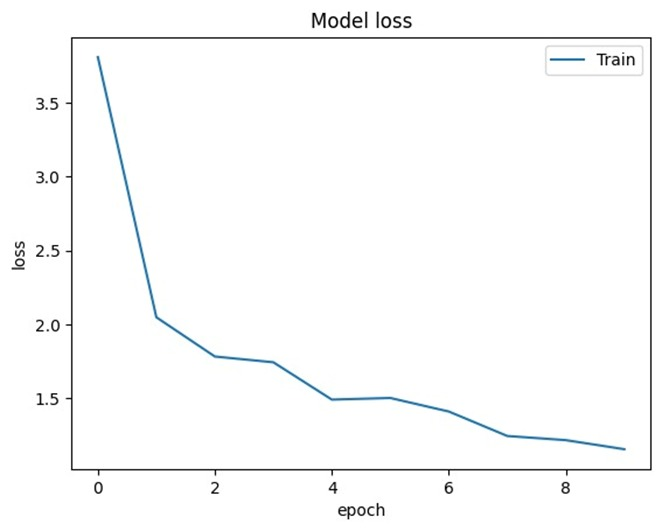
\includegraphics[width=\linewidth]{images/3.4.2.jpeg}
     
     
     \caption{}     \label{fig:my_label} 
    \end{figure}\\
\pagebreak
\linebreak
Figure 8 illustrates the accuracy of the initial phase of our project. During this phase, we developed a CNN model from scratch using the mnist dataset.

\begin{figure}[h]
    \centering
    
    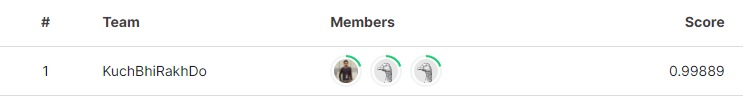
\includegraphics[width=\linewidth]{images/Score.jpeg}
     
     
     \caption{}     \label{fig:my_label} 
    \end{figure}\\

\linebreak
\linebreak
\linebreak
%\pagebreak

Figure 9 presents the model accuracy achieved during the second phase of our project. In this stage, we employed a pre-trained VGG-16 model with its previous weights and biases, utilizing the Adam optimizer. The training data used for this phase came from the StreetNumbers dataset.

\begin{figure}[h]
    \centering
    
    
\includegraphics[width=\linewidth]{images/Score 2.jpeg}
     
     
     \caption{}     \label{fig:my_label} 
    \end{figure}\\
\linebreak
\linebreak
\begin{figure}[h]
    \centering
    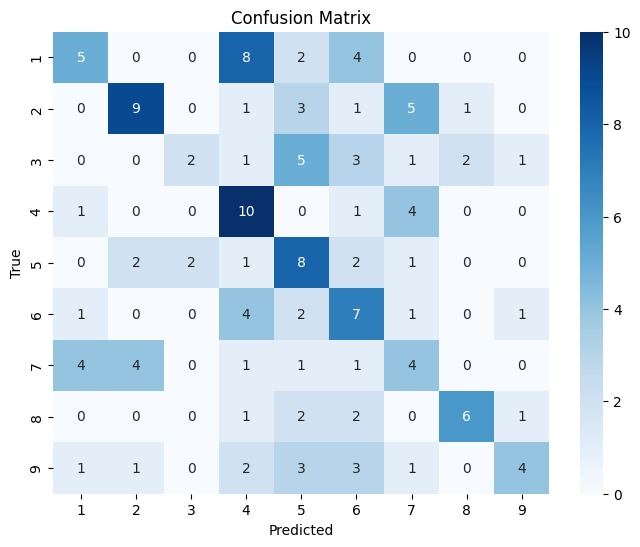
\includegraphics[width=\linewidth]{images/Confusion Matrix.jpeg}
     
     
     \caption{}     \label{fig:my_label} 
    \end{figure}\\

\Pagebreak
\section{Discussion}

\subsection{Results Discussion}

In the context of neural network training, using a more aggressive learning rate entails utilizing a larger step size when updating the model's parameters during each optimization iteration, potentially leading to faster convergence but also an increased risk of overshooting optimal values. Employing a medium batch size of 16 involves dividing the training dataset into subsets of 16 samples each, and updating the model based on the average gradient computed from these subsets, striking a balance between computational efficiency and noise in gradient estimation. Opting for the Adam optimizer involves utilizing a more sophisticated optimization algorithm compared to traditional stochastic gradient descent (SGD), as Adam incorporates adaptive learning rates for each parameter, which can lead to improved convergence in complex optimization landscapes. Overall, these choices collectively aim to accelerate training by utilizing a larger learning rate and leveraging the benefits of both a medium batch size and the advanced Adam optimizer, potentially facilitating quicker convergence and enhanced optimization outcomes.
\linebreak

Figure 11 showcases the three most successful iterations of our model training, providing insights into our training accuracy, training loss in relation to epochs and batch size, as well as the optimizer used.

\begin{figure}[h]
    \centering
    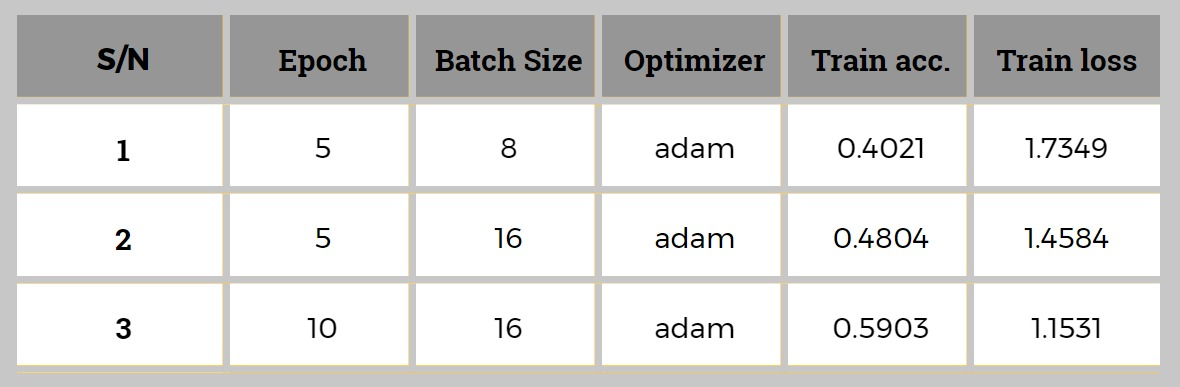
\includegraphics[width=\linewidth]{images/4.1.1.jpeg}
     
     
     \caption{}     \label{fig:my_label} 
    \end{figure}\\
%\pagebreak

\subsection{Positives and Key Findings}

The neural network has successfully acquired the ability to learn from the data it has been exposed to, demonstrating effective generalization as it avoids overfitting, wherein it captures noise instead of genuine patterns. The process of hyperparameter optimization, involving the systematic tuning of parameters that influence the network's behavior, has produced positive results for our system. This is evidenced by a substantial performance gain of 10 percentage points, elevating the network's output from a 49\% accuracy level to an improved 59\% accuracy, showcasing the efficacy of the chosen hyperparameter configurations in enhancing the model's overall performance.
\linebreak
 \newline → Network learns
\begin{itemize}
    \item Network does not overfit
    \item hyperparameter optimization has proven effective for us
(from 49\% to 59\% performance gain)
\end{itemize}


\subsection{Limitations}
The dataset used for training and testing the model is constrained by a finite number of images, potentially affecting the model's performance due to a limited variety of examples to learn from. This scarcity can hinder the network's capacity to generalize effectively to new, unseen data, as it may struggle to recognize patterns and variations that would be present in a more extensive dataset.

In addition to these challenges, the quality of the dataset itself poses a concern as it has not undergone thorough cleaning procedures. This means that the dataset includes images with multiple numbers present in a single frame, making it difficult for the model to correctly identify individual digits. Furthermore, the dataset contains images captured from a distance, introducing potential distortion and variations that are not representative of close-up images, and low-resolution images that lack the clarity necessary for accurate recognition. These suboptimal data quality issues collectively undermine the model's potential performance, as it struggles to learn from noisy, unclear, and unconventional data representations, thus highlighting the critical importance of data curation and preprocessing in achieving desirable outcomes.

%\pagebreak
\section{Conclusion}
In summary, our semester-long journey through deep learning has been nothing less than enlightening and fulfilling. Our exploration of the intricacies of neural networks, convolutional neural networks (CNNs), and their applications in computer vision has provided us with a deep understanding of the underlying mechanisms that underlie these innovative techniques.

Through diligent study and practical hands-on experience, we not only grasped the theoretical foundations but also translated this knowledge into practical know-how expertise. The Python library Keras became our canvas and allowed us to brush strokes of innovation as we implemented various neural network architectures. Engaging in these practical exercises has strengthened our understanding of the inner workings of neural networks, thereby enhancing our expertise in the subject matter.

A significant milestone in our journey was our exploration of transfer learning, a technique that significantly boosted the accuracy of our models. Leveraging pre-trained models like VGG-16 allowed us to showcase our versatility and grasp the immense potential of harnessing existing knowledge to address unique and challenging tasks.

In this dynamic and rapidly evolving field, the importance and significance of data augmentation cannot be understated. As we delved into this process, we recognized how manipulating and diversifying our data facilitated the robustness and generalization of our models, an indispensable capability skill in our pursuit of excellence.

As we complete our research, we realize that we have the technical know-how to create, train, and improve neural networks as well as an undying curiosity to learn more. Our continued development in the field of deep learning will be fueled by the foundations we've built and the insights we've obtained. We leave this chapter with the ability to decipher intricacies and the zeal to explore uncharted territory in the always changing field of artificial intelligence.

%\pagebreak
\section*{Submission of project works xAI-Proj}
\subsection*{Team Contribution}
\textbf{Shehroz Shafiq Khan}
\begin{itemize}
    \item In-depth research and usage of different Python libraries for data manipulation and data visualization.
    \item Explored various Keras modules and layers, selecting those that best suited the project's requirements.
    \item Implemented a range of CNN architectures using Keras, tailoring each model to the specific requirements for both MNIST and StreetNumbers datasets.
    \item Integrated Keras's transfer learning capabilities, incorporating pre-trained CNN models like VGG16 to assess its suitability for the street number recognition task.
    \item Implemented data augmentation techniques to artificially expand the training dataset and conducted experiments to assess the impact of data augmentation on reducing overfitting.
    \item Led the team's efforts in physically visiting various neighborhoods and recording images of street house numbers for the dataset.
\end{itemize}
%\pagebreak
\linebreak
\newline \textbf{Hafiz Ahmer Saeed Khan}
\begin{itemize}
    \item Research on different CNN models and in-depth study of their architectures that led to the selection of specific CNN models used in the project.
    \item Implemented hyperparameter tuning to optimize the model's learning rate, batch size, and other parameters crucial for achieving high accuracy.
    \item Compiled the final project report, summarizing the methodology, results, and insights from our CNN model analysis.
    \item Put together the presentations and deliverables in all phases of the project.
    \item Visited different neighborhoods to collect images of street house numbers for the dataset.
\end{itemize}
\pagebreak
\newline \textbf{Muhammad Junaid} 
\begin{itemize}
    \item Research on different Computer Vision based problems and their solutions.
    \item Developed custom evaluation metrics specific to the street number recognition task, such as precision-recall curves and confusion matrices, to gain deeper insights into model performance.
    \item Explored different cloud-based technologies for model training, such as GCP and Google Colab to utilize cloud-based GPUs and TPUs for efficient training of the diverse CNN models, optimizing resource utilization.
    \item Collaborated with other team members to optimize model efficiency.
    \item Compiled the final project documentation.
    \item Visited different neighborhoods to collect images of street house numbers for the dataset.
\end{itemize}
\textbf{GIT repository : \url{https://github.com/shehrozshafiqkh/xAI-deep-learning}} 
\vspace{140 mm}
\pagebreak

\section*{References}

1- Tyler Folkman: How To Get Started with Deep Learning 
 \newline(\url{https://towardsdatascience.com/how-to-get-started-with-deep-learning-1f4e9f9b221e})
 \linebreak
\newline 2- Purva Huilgol : Getting into Deep Learning \newline (\url{https://www.analyticsvidhya.com/blog/2020/03/deep-learning-5-things-to-know/})
\linebreak
\newline 3- Jason Brownlee : Transfer Learning in Keras with Computer Vision Models (\url{https://machinelearningmastery.com/how-to-use-transfer-learning-when-developing-convolutional-neural-network-models/})
\linebreak
\newline 4- Jason Brownlee : Your First Deep Learning Project in Python with Keras Step-by-Step \newline (\url{https://machinelearningmastery.com/tutorial-first-neural-network-python-keras/})
\linebreak
\newline 5- Derrick Mwiti : A Practical Tutorial With Examples for Images and Text in Keras \newline (\url{https://neptune.ai/blog/transfer-learning-guide-examples-for-images-and-text-in-keras})
\linebreak
\newline 6- Adrian Rosebrock : Transfer Learning with Keras and Deep Learning \newline (\url{https://pyimagesearch.com/2019/05/20/transfer-learning-with-keras-and-deep-learning/})
\linebreak
\newline 7- Introduction to Keras \newline (\url{https://keras.io/getting_started/})
\linebreak
\newline 8- Fuzhen Zhuang, Zhiyuan Qi, Keyu Duan, Dongbo Xi, Yongchun Zhu, Hengshu Zhu, Hui Xiong, Qing He : A Comprehensive Survey on Transfer Learning \newline(\url{https://arxiv.org/abs/1911.02685})



%\bibliography{bibliography}
%\bibliographystyle{abbrvnat}


%%%%%%%%%%%%%%%%%%%%%%%%%%%%%%%%%%%%%%%%%%%%%%%%%%%%%%%%%%%%%%%%%%%%%%%%%%%%%%%%%%%%%%%%%%%%%%%%%%%%
%% Declaration of Authorship
%%%%%%%%%%%%%%%%%%%%%%%%%%%%%%%%%%%%%%%%%%%%%%%%%%%%%%%%%%%%%%%%%%%%%%%%%%%%%%%%%%%%%%%%%%%%%%%%%%%%
\pagebreak

\section*{Declaration of Authorship}
All final papers have to include the following ‘Declaration of Authorship’:

{\parindent 0cm
%%%%%%%%%%%%%%%%%%%%%%%%%%German%%%%%%%%%%%%%%%%%%%%%%%%%%%%%%
\section*{Declaration of Authorship}
Ich erkläre hiermit gemäß § 9 Abs. 12 APO, dass ich die vorstehende Projektarbeit selbstständig verfasst und keine anderen als die angegebenen Quellen und Hilfsmittel benutzt habe. Des Weiteren erkläre ich, dass die digitale Fassung der gedruckten Ausfertigung der Projektarbeit ausnahmslos in Inhalt und Wortlaut entspricht und zur Kenntnis genommen wurde, dass diese digitale Fassung einer durch Software unterstützten, anonymisierten Prüfung auf Plagiate unterzogen werden kann.\\
\vspace{2\baselineskip}
  
Bamberg, \today

\rule[0.5em]{14em}{0.5pt} \hspace{0.25\linewidth}\rule[0.5em]{14em}{0.5pt}
\vspace{1em}
\hspace{4em} (Place, Date) \hspace{0.51\linewidth} (Signature)

Bamberg, \today

\rule[0.5em]{14em}{0.5pt} \hspace{0.25\linewidth}\rule[0.5em]{14em}{0.5pt}
\vspace{1em}
\hspace{4em} (Place, Date) \hspace{0.51\linewidth} (Signature)

Bamberg, \today

\rule[0.5em]{14em}{0.5pt} \hspace{0.25\linewidth}\rule[0.5em]{14em}{0.5pt}
\vspace{1em}
\hspace{4em} (Place, Date) \hspace{0.51\linewidth} (Signature)

%Bamberg, \today

%\rule[0.5em]{14em}{0.5pt} \hspace{0.25\linewidth}\rule[0.5em]{14em}{0.5pt}
%\vspace{1em}
%\hspace{4em} (Place, Date) \hspace{0.51\linewidth} (Signature)
}



%%%%%%%%%%%%%%%%%%%%%%%%%%%%%%%%%%%%%%%%%%%%%%%%%%%%%%%%%%%%


%%%%%%%%%%%%%%%%%%%%%%%%%%%%%%%%%%%%%%%%%%%%%%%%%%%%%%%%%%%%




\end{document}
